\documentclass{beamer}
\usetheme[sectionpage=progressbar, subsectionpage=progressbar, numbering=fraction, progressbar=foot, block=fill, background=light]{metropolis}
\usepackage{appendixnumberbeamer}
\usepackage{textpos}
\usepackage{booktabs}
\usepackage[scale=2]{ccicons}

\usepackage{pgfplots}
\usepgfplotslibrary{dateplot}
\usetikzlibrary{backgrounds}
\usepackage{xspace}
\newcommand{\themename}{\textbf{\textsc{metropolis}}\xspace}
\title{Attention based models in End-to-End ASR}
\subtitle{Exploration of Attention in ESPNET toolkit}
\date{\today}
\author{Shreekantha Nadig}
\institute{International Institute of Information Technology - Bangalore}
%\titlegraphic{\hfill\includegraphics[height=1.5cm]{logo.pdf}}

\usepackage{tikz}
\usetikzlibrary{shapes,shadows,arrows,patterns, matrix}

\tikzstyle{line} = [draw, -latex']
\tikzstyle{round} = [draw, circle, fill=black!30, minimum size=4em, node distance=4em, font=\fontsize{30}{10}\selectfont]
\tikzstyle{mlp_enc} = [rectangle, draw, fill=red!50, text width=2cm, minimum height=5em, text centered, node distance=10em, font=\fontsize{20}{10}\selectfont]
\tikzstyle{mlp_att} = [rectangle, draw, fill=green!50, text width=2cm, minimum height=5em, text centered, node distance=10em, font=\fontsize{20}{10}\selectfont]
\tikzstyle{mlp_dec} = [rectangle, draw, fill=blue!50, text width=2cm, minimum height=5em, text centered, node distance=10em, font=\fontsize{20}{10}\selectfont]
\tikzstyle{enc_h} = [rectangle, draw,  pattern=horizontal lines, pattern color=red!60, text width=1cm, minimum height=10em, minimum width=3em, text centered, node distance=10em, font=\fontsize{25}{10}\selectfont]
\tikzstyle{atts} = [rectangle, draw,  pattern=horizontal lines, pattern color=green!70, text width=1cm, minimum height=10em, minimum width=3em, text centered, node distance=10em, font=\fontsize{20}{10}\selectfont]
\tikzstyle{dec_z} = [rectangle, draw,  pattern=horizontal lines, pattern color=blue!60, text width=1cm, minimum height=10em, minimum width=3em, text centered, node distance=10em, font=\fontsize{20}{10}\selectfont]
\tikzstyle{cnn} = [rectangle, draw,  pattern=crosshatch, pattern color=red!50!blue!50, text width=2cm, minimum height=5em, text centered, node distance=10em, font=\fontsize{20}{10}\selectfont]
\tikzstyle{box} = [rectangle, draw,  fill=blue!20, text width=3cm, minimum height=5em, minimum width=3em, text centered, node distance=10em, font=\fontsize{20}{10}\selectfont]

\begin{document}
	\addtobeamertemplate{frametitle}{}{%
		\begin{textblock*}{100mm}(.97\textwidth,-1cm)
			{
\includegraphics[width=2.5em]{iiitb_logo.png}}
		\end{textblock*}}

%\maketitle

\begin{frame}[fragile]{Coverage mechanism Attention}
\begin{center}
	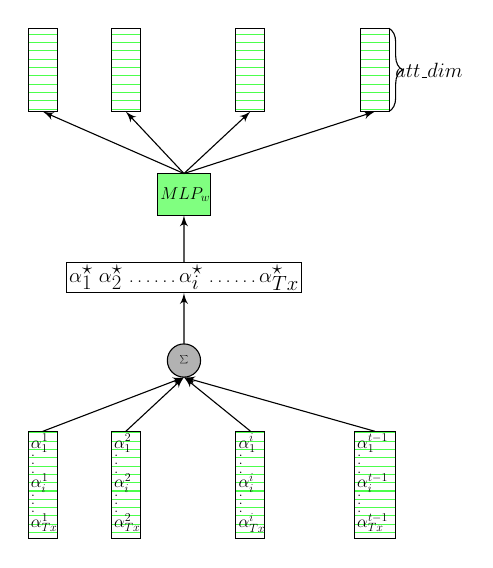
\begin{tikzpicture}[scale=0.3, every node/.style={transform shape, font=\fontsize{40}{40}\selectfont}]
		\node [atts, minimum height = 12em] (alpha1) {$\alpha_{1}^{1}$ \newline . \newline . \newline . \newline $\alpha_{i}^{1}$ \newline . \newline . \newline . \newline $\alpha_{Tx}^{1}$ \newline};
		\node [atts, right of=alpha1, minimum height = 12em] (alpha2) {$\alpha_{1}^{2}$ \newline . \newline . \newline . \newline $\alpha_{i}^{2}$ \newline . \newline . \newline . \newline $\alpha_{Tx}^{2}$ \newline};
		\node [atts, right of=alpha2, node distance = 15em, minimum height = 12em] (alphai) {$\alpha_{1}^{i}$ \newline . \newline . \newline . \newline $\alpha_{i}^{i}$ \newline . \newline . \newline . \newline $\alpha_{Tx}^{i}$ \newline};
		\node [atts, right of=alphai, node distance = 15em, minimum height = 12em, text width = 1.5cm] (alphaTx) {$\alpha_{1}^{t-1}$ \newline . \newline . \newline . \newline $\alpha_{i}^{t-1}$ \newline . \newline . \newline . \newline $\alpha_{Tx}^{t-1}$ \newline};
		\node [round, above of = alphai, xshift = -8em, node distance = 15em] (sum) {$\sum$};
		\path [line] (alpha1.north) to (sum.south);
		\path [line] (alpha2.north) to (sum.south);
		\path [line] (alphai.north) to (sum.south);
		\path [line] (alphaTx.north) to (sum.south);
		\node [draw, above of = sum, node distance = 10em] (alphastar) {$\alpha_{1}^{\star}$ $\alpha_{2}^{\star}$ \dots \dots $\alpha_{i}^{\star}$ \dots \dots $\alpha_{Tx}^{\star}$};
		\node [mlp_att, above of = alphastar, node distance = 10em] (mlp_w) {$MLP_{w}$};
		
		\node [atts, above of = alpha1, node distance = 50em] (alpha1) {};
		\node [atts, right of=alpha1] (alpha2) {};
		\node [atts, right of=alpha2, node distance = 15em] (alphai) {};
		\node [atts, right of=alphai, node distance = 15em] (alphaTx) {};
		
		
		\draw [decorate,decoration={brace,amplitude=5pt, raise=0.5em}] (alphaTx.90) -- (alphaTx.-90) node [black,midway, xshift=6.5em] {\fontsize{25}{10}\selectfont $att\_dim$};
		
		\path [line] (sum.north) to (alphastar.south);
		\path [line] (alphastar.north) to (mlp_w.south);
		\path [line] (mlp_w.north) to (alpha1.south);
		\path [line] (mlp_w.north) to (alpha2.south);
		\path [line] (mlp_w.north) to (alphai.south);
		\path [line] (mlp_w.north) to (alphaTx.south);
		
		
	\end{tikzpicture}
\end{center}
\end{frame}

\begin{frame}[fragile]{Coverage mechanism Attention}
\begin{center}
	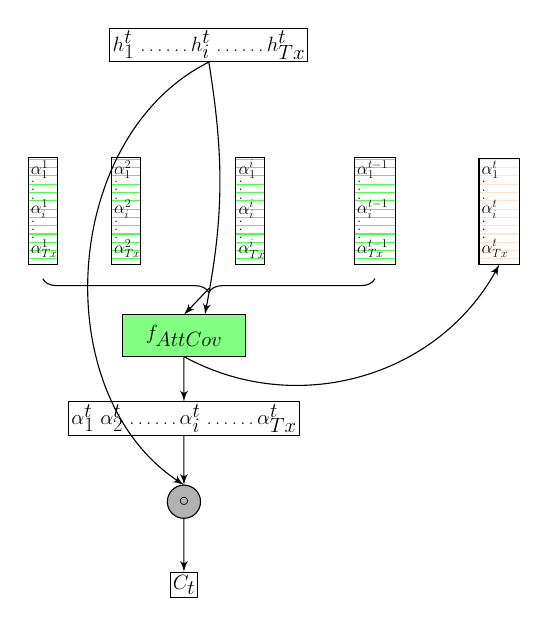
\begin{tikzpicture}[scale=0.3, every node/.style={transform shape, font=\fontsize{40}{40}\selectfont}]
	\node [draw] (ht) {$h_{1}^{t}$ \dots \dots $h_{i}^{t}$ \dots \dots $h_{Tx}^{t}$};
		
	\node [atts, below of = ht, xshift=-20em, node distance = 20em] (alpha1) {$\alpha_{1}^{1}$ \newline . \newline . \newline . \newline $\alpha_{i}^{1}$ \newline . \newline . \newline . \newline $\alpha_{Tx}^{1}$ \newline};
	\node [atts, right of=alpha1, minimum height = 12em] (alpha2) {$\alpha_{1}^{2}$ \newline . \newline . \newline . \newline $\alpha_{i}^{2}$ \newline . \newline . \newline . \newline $\alpha_{Tx}^{2}$ \newline};
	\node [atts, right of=alpha2, node distance = 15em, minimum height = 12em] (alphai) {$\alpha_{1}^{i}$ \newline . \newline . \newline . \newline $\alpha_{i}^{i}$ \newline . \newline . \newline . \newline $\alpha_{Tx}^{i}$ \newline};
	\node [atts, right of=alphai, node distance = 15em, minimum height = 12em, text width = 1.5cm] (alphaTx) {$\alpha_{1}^{t-1}$ \newline . \newline . \newline . \newline $\alpha_{i}^{t-1}$ \newline . \newline . \newline . \newline $\alpha_{Tx}^{t-1}$ \newline};
	
	\node [mlp_att, below of= alphai, xshift=-8em, font=\fontsize{60}{60}\selectfont, text width = 5cm, node distance = 15em] (attcov) {$f_{AttCov}$};
	
	\node [draw, below of = attcov, node distance = 10em] (alphastar) {$\alpha_{1}^{t}$ $\alpha_{2}^{t}$ \dots \dots $\alpha_{i}^{t}$ \dots \dots $\alpha_{Tx}^{t}$};
	
	\draw [decorate,decoration={brace,amplitude=5pt, raise=0.5em, mirror}] (alpha1.south) -- (alphaTx.south) node [black,midway, yshift = -2.5em] (t) {};
	
	\path [line] (t.south) to (attcov.north);
	
	\path [line] (ht.south) to [bend left=10] (attcov.45);
	\path [line] (attcov.south) to (alphastar);
	
	\node [atts, right of=alphaTx,pattern color= orange!20, node distance = 15em, minimum height = 12em, text width = 1.5cm] (alphat) {$\alpha_{1}^{t}$ \newline . \newline . \newline . \newline $\alpha_{i}^{t}$ \newline . \newline . \newline . \newline $\alpha_{Tx}^{t}$ \newline};
	
	\path [line] (attcov.south) to [bend right=45](alphat.south);
	\node [round, below of=alphastar, node distance = 10em] (dot) {$\circ$};
	\path [line] (ht.south) to [bend right=60](dot.north);
	\path [line] (alphastar.south) to (dot.north);
	
	\node [draw, below of = dot, node distance = 10em] (ct) {$C_{t}$};
	
	\path [line] (dot.south) to (ct.north);
	
	\end{tikzpicture}
\end{center}
\end{frame}


	\begin{frame}[fragile]{Coverage mechanism Attention}
	\begin{center}
		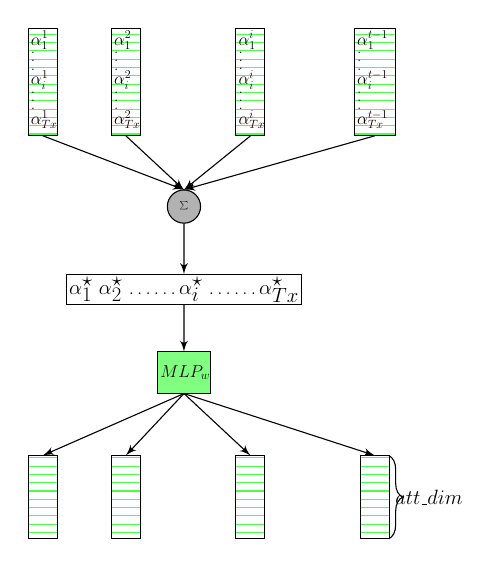
\begin{tikzpicture}[scale=0.3, every node/.style={transform shape, font=\fontsize{40}{40}\selectfont}]
			\node [atts, minimum height = 12em] (alpha1) {$\alpha_{1}^{1}$ \newline . \newline . \newline . \newline $\alpha_{i}^{1}$ \newline . \newline . \newline . \newline $\alpha_{Tx}^{1}$ \newline};
			
			\node [atts, right of=alpha1, minimum height = 12em] (alpha2) {$\alpha_{1}^{2}$ \newline . \newline . \newline . \newline $\alpha_{i}^{2}$ \newline . \newline . \newline . \newline $\alpha_{Tx}^{2}$ \newline};
			
			\node [atts, right of=alpha2, node distance = 15em, minimum height = 12em] (alphai) {$\alpha_{1}^{i}$ \newline . \newline . \newline . \newline $\alpha_{i}^{i}$ \newline . \newline . \newline . \newline $\alpha_{Tx}^{i}$ \newline};
			
			\node [atts, right of=alphai, node distance = 15em, minimum height = 12em, text width = 1.5cm] (alphaTx) {$\alpha_{1}^{t-1}$ \newline . \newline . \newline . \newline $\alpha_{i}^{t-1}$ \newline . \newline . \newline . \newline $\alpha_{Tx}^{t-1}$ \newline};
			
			\node [round, below of = alphai, xshift = -8em, node distance = 15em] (sum) {$\sum$};
			\path [line] (alpha1.south) to (sum.north);
			\path [line] (alpha2.south) to (sum.north);
			\path [line] (alphai.south) to (sum.north);
			\path [line] (alphaTx.south) to (sum.north);
			
			\node [draw, below of = sum, node distance = 10em] (alphastar) {$\alpha_{1}^{\star}$ $\alpha_{2}^{\star}$ \dots \dots $\alpha_{i}^{\star}$ \dots \dots $\alpha_{Tx}^{\star}$};
			\node [mlp_att, below of = alphastar, node distance = 10em] (mlp_w) {$MLP_{w}$};
			
			\node [atts, below of = alpha1, node distance = 50em] (alpha1) {};
			\node [atts, right of=alpha1] (alpha2) {};
			\node [atts, right of=alpha2, node distance = 15em] (alphai) {};
			\node [atts, right of=alphai, node distance = 15em] (alphaTx) {};
			
			
			\draw [decorate,decoration={brace,amplitude=5pt, raise=0.5em}] (alphaTx.90) -- (alphaTx.-90) node [black,midway, xshift=6.5em] {\fontsize{25}{10}\selectfont $att\_dim$};
			
			\path [line] (sum.south) to (alphastar.north);
			\path [line] (alphastar.south) to (mlp_w.north);
			\path [line] (mlp_w.south) to (alpha1.north);
			\path [line] (mlp_w.south) to (alpha2.north);
			\path [line] (mlp_w.south) to (alphai.north);
			\path [line] (mlp_w.south) to (alphaTx.north);
		\end{tikzpicture}
	\end{center}
\end{frame}	

\begin{frame}[fragile]{Coverage mechanism Attention}
\begin{center}
	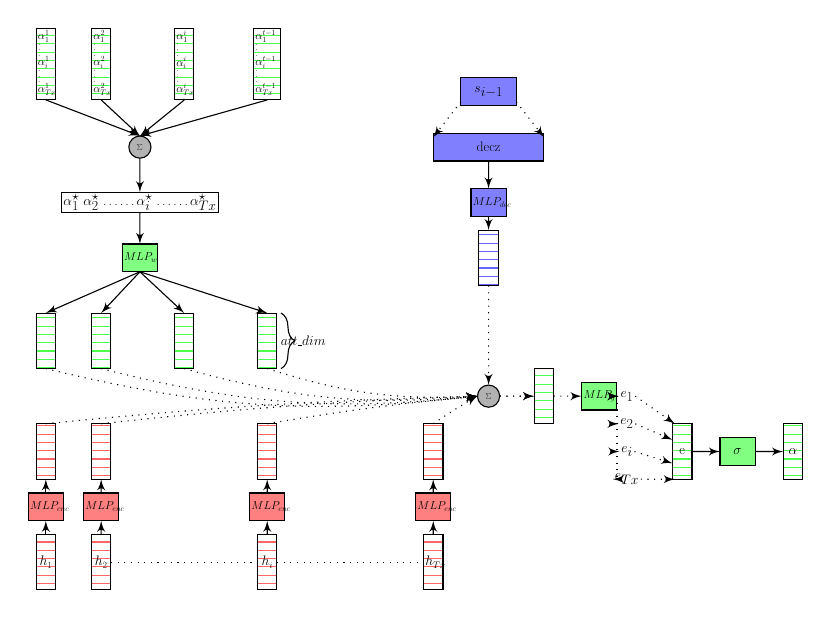
\begin{tikzpicture}[scale=0.2, every node/.style={transform shape, font=\fontsize{40}{40}\selectfont}]
		
				\node [enc_h] (h1) {$h_{1}$};
		\node [enc_h,right of = h1] (h2) {$h_{2}$};
		\node [enc_h,right of = h2, node distance = 30em] (hi) {$h_{i}$};
		\node [enc_h,right of = hi, node distance = 30em] (hTx) {$h_{Tx}$};
		\draw [dotted] (h2.east) to (hi.west);
		\draw [dotted] (hi.east) to (hTx.west);
		
		
		\node [mlp_enc, above of = h1, node distance = 10em] (mlp1) {$MLP_{enc}$};
		\path [line] (h1.north) to (mlp1.south);
		\node [enc_h, above of = mlp1] (he1) {};
		\path [line] (mlp1.north) to (he1.south);
		
		
		\node [mlp_enc, above of = h2, node distance = 10em] (mlp2) {$MLP_{enc}$};
		\path [line] (h2.north) to (mlp2.south);
		\node [enc_h, above of = mlp2] (he2) {};
		\path [line] (mlp2.north) to (he2.south);
		
		
		\node [mlp_enc, above of = hi, node distance = 10em] (mlpi) {$MLP_{enc}$};
		\path [line] (hi.north) to (mlpi.south);
		\node [enc_h, above of = mlpi] (hei) {};
		\path [line] (mlpi.north) to (hei.south);
		
		
		\node [mlp_enc, above of = hTx, node distance = 10em] (mlpTx) {$MLP_{enc}$};
		\path [line] (hTx.north) to (mlpTx.south);
		\node [enc_h, above of = mlpTx] (heTx) {};
		\path [line] (mlpTx.north) to (heTx.south);
		
		
		\node [atts, minimum height = 12em,  above of=he1, node distance = 70em] (alpha1) {$\alpha_{1}^{1}$ \newline . \newline . \newline . \newline $\alpha_{i}^{1}$ \newline . \newline . \newline . \newline $\alpha_{Tx}^{1}$ \newline};
		
		\node [atts, right of=alpha1, minimum height = 12em] (alpha2) {$\alpha_{1}^{2}$ \newline . \newline . \newline . \newline $\alpha_{i}^{2}$ \newline . \newline . \newline . \newline $\alpha_{Tx}^{2}$ \newline};
		
		\node [atts, right of=alpha2, node distance = 15em, minimum height = 12em] (alphai) {$\alpha_{1}^{i}$ \newline . \newline . \newline . \newline $\alpha_{i}^{i}$ \newline . \newline . \newline . \newline $\alpha_{Tx}^{i}$ \newline};
		
		\node [atts, right of=alphai, node distance = 15em, minimum height = 12em, text width = 1.5cm] (alphaTx) {$\alpha_{1}^{t-1}$ \newline . \newline . \newline . \newline $\alpha_{i}^{t-1}$ \newline . \newline . \newline . \newline $\alpha_{Tx}^{t-1}$ \newline};
		
		\node [round, below of = alphai, xshift = -8em, node distance = 15em] (sum) {$\sum$};
		\path [line] (alpha1.south) to (sum.north);
		\path [line] (alpha2.south) to (sum.north);
		\path [line] (alphai.south) to (sum.north);
		\path [line] (alphaTx.south) to (sum.north);
		
		\node [draw, below of = sum, node distance = 10em] (alphastar) {$\alpha_{1}^{\star}$ $\alpha_{2}^{\star}$ \dots \dots $\alpha_{i}^{\star}$ \dots \dots $\alpha_{Tx}^{\star}$};
		\node [mlp_att, below of = alphastar, node distance = 10em] (mlp_w) {$MLP_{w}$};
		
		\node [atts, below of = alpha1, node distance = 50em] (alpha1) {};
		\node [atts, right of=alpha1] (alpha2) {};
		\node [atts, right of=alpha2, node distance = 15em] (alphai) {};
		\node [atts, right of=alphai, node distance = 15em] (alphaTx) {};
		
		
		\draw [decorate,decoration={brace,amplitude=5pt, raise=0.5em}] (alphaTx.90) -- (alphaTx.-90) node [black,midway, xshift=6.5em] {\fontsize{25}{10}\selectfont $att\_dim$};
		
		\path [line] (sum.south) to (alphastar.north);
		\path [line] (alphastar.south) to (mlp_w.north);
		\path [line] (mlp_w.south) to (alpha1.north);
		\path [line] (mlp_w.south) to (alpha2.north);
		\path [line] (mlp_w.south) to (alphai.north);
		\path [line] (mlp_w.south) to (alphaTx.north);
	
		\node [round, above of=heTx, node distance=10em, xshift=10em] (sum1) {$\sum$};
		
		\path [line, dotted] (he1.north) to [bend left=2] (sum1.west);
		\path [line, dotted] (he2.north) to [bend left=2] (sum1.west);
		\path [line, dotted] (hei.north) to [bend left=2] (sum1.west);
		\path [line, dotted] (heTx.north) to [bend left=2] (sum1.west);
		
		
		\node [mlp_dec, right of = mlp_w, node distance = 63em, minimum width = 10em, yshift=30em, font=\fontsize{40}{10}\selectfont] (sim1) {$s_{i-1}$};
		\node [mlp_dec, below of=sim1, minimum width = 20em, font=\fontsize{40}{10}\selectfont] (dec_z) {decz};
		\path [line, dotted] (sim1.200) to (dec_z.170);
		\path [line, dotted] (sim1.-20) to (dec_z.10);
		\node [mlp_dec, below of=dec_z, node distance = 10em] (mlp_dec) {$MLP_{dec}$};
		\path [line] (dec_z) to (mlp_dec);
		\node [dec_z, below of = mlp_dec] (decz_enc) {};
		\path [line] (mlp_dec) to (decz_enc);
		
		\path [line, dotted] (decz_enc.south) to (sum1.north);
		
%		\path [line, dotted] (ht.east) to [bend left=10] (sum1.110);
		\node [atts, right of=sum1, node distance = 10em] (asdf) {};
		\node [mlp_att, right of=asdf] (mlpg) {$MLP_{g}$};
		\node [right of=mlpg, node distance=5em, font=\fontsize{40}{10}\selectfont] (e1) {$e_1$};
		
		\node [below of=e1, node distance=5em, font=\fontsize{40}{10}\selectfont] (e2) {$e_2$};
		
		\node [below of=e2, node distance=5em, font=\fontsize{40}{10}\selectfont] (ei) {$e_i$};
		
		\node [below of=ei, node distance=5em, font=\fontsize{40}{10}\selectfont] (eTx) {$e_{Tx}$};
		
		\node [atts, right of=ei, font=\fontsize{40}{10}\selectfont] (e) {e};
		
		\path [line, dotted] (e1.east) to (e.105);
		\path [line, dotted] (e2.east) to (e.130);
		\path [line, dotted] (ei.east) to (e.-130);
		\path [line, dotted] (eTx.east) to (e.-105);
		
		\node [mlp_att, right of=e, font=\fontsize{40}{10}\selectfont] (sm) {$\sigma$};
		\path [line] (e.east) to (sm.west);
		
		
		\node [atts, right of=sm, font=\fontsize{40}{10}\selectfont] (alphas) {$\alpha$};
		\path [line] (sm.east) to (alphas.west);
		
		\path [line, dotted] (sum1.east) to (asdf.west);
		\path [line, dotted] (sum1.east) to (asdf.west);
		\path [line, dotted] (asdf.east) to (mlpg.west);
		\path [line, dotted] (mlpg.east) to (e1.west);
		\path [line, dotted] (mlpg.east) to (e1.west);
		\path [line, dotted] (mlpg.east) |- (e2.west);
		\path [line, dotted] (mlpg.east) |- (ei.west);
		\path [line, dotted] (mlpg.east) |- (eTx.west);
		
		\path [line, dotted] (alpha1.south) to [bend right=10] (sum1.west);
		\path [line, dotted] (alpha2.south) to [bend right=10] (sum1.west);
		\path [line, dotted] (alphai.south) to [bend right=10] (sum1.west);
		\path [line, dotted] (alphaTx.south) to [bend right=10] (sum1.west);
	\end{tikzpicture}
\end{center}
\end{frame}
\end{document}